% This file was created by matlab2tikz.
%
%The latest updates can be retrieved from
%  http://www.mathworks.com/matlabcentral/fileexchange/22022-matlab2tikz-matlab2tikz
%where you can also make suggestions and rate matlab2tikz.
%
\definecolor{mycolor1}{rgb}{0.00000,0.44700,0.74100}%
\definecolor{mycolor2}{rgb}{0.85000,0.32500,0.09800}%
\definecolor{mycolor3}{rgb}{0.92900,0.69400,0.12500}%
\definecolor{mycolor4}{rgb}{0.49400,0.18400,0.55600}%
\definecolor{mycolor5}{rgb}{0.46600,0.67400,0.18800}%
\definecolor{mycolor6}{rgb}{0.30100,0.74500,0.93300}%
%
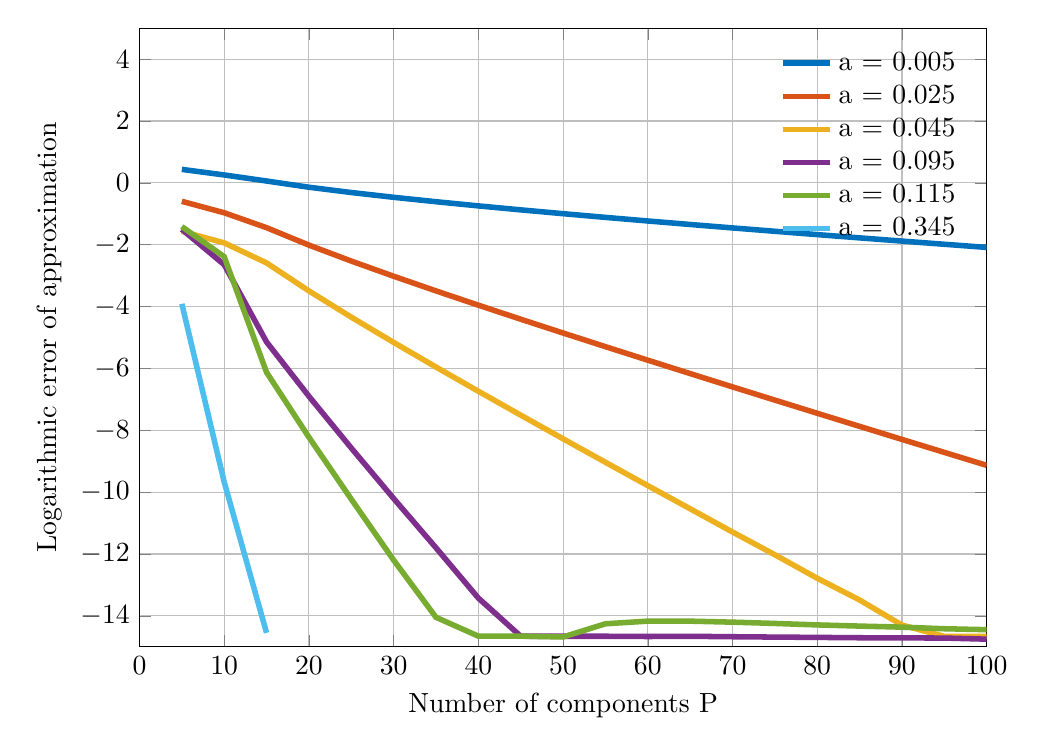
\begin{tikzpicture}

\begin{axis}[%
width=4.236in,
height=3.093in,
at={(1.043in,0.954in)},
scale only axis,
unbounded coords=jump,
xmin=0,
xmax=100,
xlabel={Number of components P},
xmajorgrids,
ymin=-15,
ymax=5,
ylabel={Logarithmic error of approximation},
ymajorgrids,
axis background/.style={fill=white},
legend style={legend cell align=left,align=left,fill=none,draw=none}
]
\addplot [color=mycolor1,solid,line width=2.0pt]
  table[row sep=crcr]{%
5	0.435979365283817\\
10	0.256092146380958\\
15	0.0601311415953336\\
20	-0.140769783158704\\
25	-0.312167561515658\\
30	-0.466482970913044\\
35	-0.609426787145836\\
40	-0.744167065513137\\
45	-0.872668008311448\\
50	-0.996243649718126\\
55	-1.11581977850619\\
60	-1.23207780575998\\
65	-1.34553307028898\\
70	-1.45658814106725\\
75	-1.56556117214105\\
80	-1.67271193200002\\
85	-1.77824962453398\\
90	-1.88235326937547\\
95	-1.98517103415603\\
100	-2.08682808589674\\
};
\addlegendentry{a = 0.005};

\addplot [color=mycolor2,solid,line width=2.0pt]
  table[row sep=crcr]{%
5	-0.596668601743884\\
10	-0.966327805568993\\
15	-1.44859648294285\\
20	-2.01194874073806\\
25	-2.52834523845899\\
30	-3.0187418829607\\
35	-3.49244047072114\\
40	-3.95445530591144\\
45	-4.40778756166549\\
50	-4.85443146401809\\
55	-5.29570817937261\\
60	-5.73265383019654\\
65	-6.16591470717832\\
70	-6.59617507118382\\
75	-7.02368861326013\\
80	-7.44908282347961\\
85	-7.87222335930877\\
90	-8.29396284771822\\
95	-8.7135981994232\\
100	-9.13261222791123\\
};
\addlegendentry{a = 0.025};

\addplot [color=mycolor3,solid,line width=2.0pt]
  table[row sep=crcr]{%
5	-1.56680711198865\\
10	-1.9399143272388\\
15	-2.58707613720019\\
20	-3.49356981832179\\
25	-4.34148392910766\\
30	-5.15781580041051\\
35	-5.95423902155605\\
40	-6.73708094312773\\
45	-7.50973813241832\\
50	-8.27513675251596\\
55	-9.03373818025513\\
60	-9.78902479342674\\
65	-10.5370994258816\\
70	-11.2882485442312\\
75	-12.0234042176922\\
80	-12.7827771742811\\
85	-13.4859051571851\\
90	-14.29735933284\\
95	-14.6623272250937\\
100	-14.6621058918815\\
};
\addlegendentry{a = 0.045};

\addplot [color=mycolor4,solid,line width=2.0pt]
  table[row sep=crcr]{%
5	-1.50050453157682\\
10	-2.64590533443851\\
15	-5.14284386092929\\
20	-6.89968242039218\\
25	-8.57248001682411\\
30	-10.2040964380133\\
35	-11.7987089717776\\
40	-13.4241061390254\\
45	-14.6574250342176\\
50	-14.6584783871581\\
55	-14.658105126748\\
60	-14.6664450399974\\
65	-14.6595304847321\\
70	-14.6738088422698\\
75	-14.6852552267502\\
80	-14.6951493333541\\
85	-14.7068841409367\\
90	-14.7115686925412\\
95	-14.7165726985756\\
100	-14.7524207967554\\
};
\addlegendentry{a = 0.095};

\addplot [color=mycolor5,solid,line width=2.0pt]
  table[row sep=crcr]{%
5	-1.41347651643263\\
10	-2.38722884182496\\
15	-6.12582944905123\\
20	-8.22381825642789\\
25	-10.2265121088053\\
30	-12.1965153953624\\
35	-14.0458071460169\\
40	-14.6552481351647\\
45	-14.6553155417244\\
50	-14.6818560846755\\
55	-14.2552956636878\\
60	-14.1696439646056\\
65	-14.170408155681\\
70	-14.2027542522096\\
75	-14.2441972197978\\
80	-14.2921245144565\\
85	-14.3297009781386\\
90	-14.3638872877249\\
95	-14.4156287608613\\
100	-14.4456050879567\\
};
\addlegendentry{a = 0.115};

\addplot [color=mycolor6,solid,line width=2.0pt]
  table[row sep=crcr]{%
5	-3.91130425213666\\
10	-9.6695755164259\\
15	-14.5481490031608\\
20	nan\\
25	nan\\
30	nan\\
35	nan\\
40	nan\\
45	nan\\
50	nan\\
55	nan\\
60	nan\\
65	nan\\
70	nan\\
75	nan\\
80	nan\\
85	nan\\
90	nan\\
95	nan\\
100	nan\\
};
\addlegendentry{a = 0.345};

\end{axis}
\end{tikzpicture}%